\documentclass[Master, ngerman, UKenglish]{scrbook}
%------------------------------------------------------------------------------
% This file contains a skeleton thesis for
% a Physics or Astronomy Institute in the University of Bonn.

% Specify the thesis type as an option: PhD, Master, Diplom, Bachelor.
% Specify the thesis stage as an option: Draft (default), Submit, Final, PILibrary.

% Specify the language(s) in the class and then use babel.
% If you need more than one language, give the default language last,
% e.g. ngerman, UKenglish for a thesis in British (UK) English where you want
% to be able to set the language to German for some part of it.

%------------------------------------------------------------------------------
% Pass TeX Live version to the package.
% Use command pdflatex --version to find out which version you are running.
% twoside=true is suitable for printing, while twoside=false is probably better for PDF version.
\usepackage[twoside=true]{ubonn-thesis}

%------------------------------------------------------------------------------
% Adjustments to standard biblatex style.
% Change option to backref=false when your thesis is ready to turn off back-referencing.
% Pass the option showurl=false to shorten your bibliography by not including url fields.
\usepackage[backref=true]{ubonn-biblatex}

\usepackage{braket}

%------------------------------------------------------------------------------
% Glossary package
% \usepackage[acronym,toc,nosuper]{glossaries}
% TikZ packages and libraries
\usepackage{tikz}
\usepackage{tikz-3dplot}
\usepackage{pgfplots}
\usetikzlibrary{positioning,shapes,arrows}
\usetikzlibrary{decorations.pathmorphing}
\usetikzlibrary{decorations.markings}
\usepackage{thesis_defs}
\usepackage{tablefootnote}
\usepackage{multirow}
\usepackage{booktabs}
%------------------------------------------------------------------------------
% Instead of colouring  links, cites, table of contents etc.
% put them in a coloured box for the screen version.
% This is probably a good idea when you print your thesis.
% \hypersetup{colorlinks=false,
%   linkbordercolor=blue,citebordercolor=magenta,urlbordercolor=darkgreen
% }

%------------------------------------------------------------------------------
% When writing your thesis it is often helpful to have the date and
% time in the output file. Comment this out for the final version.
\ifoot[\today{} \thistime]{\today{} \thistime}

% In order to check if your labels are referenced try the refcheck package
% \usepackage{refcheck}

%------------------------------------------------------------------------------
% biblatex is included by ubonn-thesis. Look there for the settings used.
% See the options for settings that can be changed easily.
% For further changes copy the \RequirePackage[...]{biblatex} here
% and include ubonn-thesis with the option biblatex=false.

% Specify the bibliography files here and not at the end!
% Use standard_refs-bibtex if you use bibtex or bibtex8
% and standard_refs-biber  if you use biber
\addbibresource{bib/thesis_refs.bib}
\addbibresource{bib/standard_refs-biber.bib}

%------------------------------------------------------------------------------
% The following definitions are used to produce the title pages
% needed at various stages
\newcommand{\thesistitle}{Study of Exotic Hadrons with Lattice QCD and Distillation}
\newcommand*{\thesisauthor}{Grant Bradley}
% \newcommand*{\thesistown}{Place of birth}
\renewcommand*{\InstituteName}{Forschungszentrum Jülich}
\renewcommand*{\inInstitute}{Jülich Supercomputing Centre}
\renewcommand*{\InstituteAddress}{\PIaddress}
% Adjust \thesisreferee...text depending on male/female referee
\newcommand*{\thesisrefereeonetext}{1.\ Gutachter}
\newcommand*{\thesisrefereeone}{Prof.\ Dr.\ Stefan Krieg}
\newcommand*{\thesisrefereetwotext}{2.\ Gutachterin}
\newcommand*{\thesisrefereetwo}{Prof.\ Dr.\ Anne Jones}
% Date when thesis was submitted (Master/Diplom)
% Year or Month, Year when thesis was submitted (PhD)
% \newcommand*{\thesissubmit}{XX.YY.2024}
% \newcommand*{\thesissubmit}{Month 2024}
% Date of thesis examination (PhD)
% \newcommand*{\thesispromotion}{XX.YY.2024}
% Month and year of the final printed version of the thesis
\newcommand*{\thesismonth}{October}
\newcommand*{\thesisyear}{2024}
% \newcommand*{\thesisnumber}{BONN-IR-2024-XXX}
% Dedication
% \newcommand*{\thesisdedication}{}

%------------------------------------------------------------------------------
% The abstract is only needed for the printed version and should be in
% English regardless of the language of the thesis
\newcommand{\thesisabstract}{%
  \begin{otherlanguage}{UKenglish}
    This is your thesis abstract. It may be in a language that is
    different from the rest of your thesis.
  \end{otherlanguage}
}

%------------------------------------------------------------------------------
% \includeonly can be used to select which chapters you want to process
% A simple \include command just inserts a \clearpage before and after the file
% Note that \includeonly can be quite picky! Do not forget to put a
% comma after the filename, otherwise it will simply be ignored!
\includeonly{%
  thesis_intro,
  thesis_spec,
  thesis_ops,
  thesis_comp,
  thesis_signal,
  thesis_future,
  thesis_appendix,
  thesis_acknowledge
}

%------------------------------------------------------------------------------
% Give a list of directories where figures can be found. Do not leave
% any spaces in the list and end the directory name with a /
\graphicspath{%
  {figs/}%
  {figs/cover/}%
  {figs/figures/}%

}

%------------------------------------------------------------------------------
% Make a glossary and a list of acronyms
% \makeglossaries

% Glossary entries
% \input{thesis_glossary}

% Draft version - add the word DRAFT on the cover pages
% Also add the date and time of compilation and turn on line numbers (if option is set).
\ifthenelse{\equal{\ThesisVersion}{Draft}}{%
  \usepackage{background}
  \backgroundsetup{contents=DRAFT, color=blue!30}
  \ifoot[\today{} \thistime]{\today{} \thistime}
  \ifthenelse{\boolean{ThesisLineno}}{\linenumbers}{}
 }

%------------------------------------------------------------------------------
\begin{document}

% Make cover and title pages
\makethesistitle

\pagestyle{scrplain}

%------------------------------------------------------------------------------
% You can add your acknowledgements here - don't forget to also add
% them to \includeonly above
%------------------------------------------------------------------------------
\chapter*{Acknowledgements}
\label{sec:ack}
%------------------------------------------------------------------------------

I would like to thank my advisor Prof.\ Dr.\ Stefan Krieg for giving me the opportunity to pursue my PhD in a beautiful topic and country. He provides endless guidance in both the research vocation and how to navigate the problems that arise when moving to a foreign country. His advice in both realms is always just a door-knock or phone call away and has made my adjustment to Germany, and the frustration-laden process of conducting research, all the more smoother.       

I also wish to thank Dr.\ Giovanni Pederiva for his tireless attention to detail with all things programming, the physics ``big picture'', and advice on how to manage my workflow in an efficient manner. His programming and HPC expertise have been a crucial factor in progressing this project forward. I am indebetted to his patience and suggestions at every step of the way. 

I would be remiss to not acknowledge the fruitful discussions with Dr.\ Evan Berkowitz; His insightful ``mini lectures'' have illuminated countless deep truths in physics and group theory that were previously unbeknownst to me. 


% You should probably use \texttt{\textbackslash chapter*} for
% acknowledgements at the beginning of a thesis and
% \texttt{\textbackslash chapter} for the end.

%%% Local Variables: 
%%% mode: latex
%%% TeX-master: "../mythesis"
%%% End: 


\tableofcontents

\mainmatter
\pagestyle{scrheadings}

% Turn off DRAFT for the following pages
\ifthenelse{\equal{\ThesisVersion}{Draft}}{%
  \backgroundsetup{contents={}}
}{}

%------------------------------------------------------------------------------
% Add your chapters here - don't forget to also add them to \includeonly above
% !TEX root = mythesis.tex

%==============================================================================
\chapter{Introduction}
\label{sec:intro}
\newcommand{\todo}[1]{\textbf{\color{red}TODO: #1}}

%==============================================================================
Quantum Chromodynamics is the SU(3) gauge field theory governing the strong force, dictating the dynamics of quarks and gluons. One can have two or three quark states, mesons and baryons, respectively, bound together by gluons. QCD phenomena are informed by two main quark correlations: confinement, whereby color forces allow $q,\bar{q}$ to be correlated into color singlets, and chiral symmetry breaking. In continuum QCD, the regime in which the coupling constant of the theory $\alpha_s$ is still small, perturbation theory can reliably be used. However, to probe the hadronic world ($\mu \leq 1 GeV$), perturbation theory ceases to be a useful tool. By discretizing Minkowski spacetime into Euclidean spacetime, we can calculate the hadron spectrum and other quantities such as matrix elements.  This non-perturbative approach is called Lattice QCD(henceforth LQCD), the only systematically improvable and regularization scheme independent method to probe the strong force. It is crucial to note that this formulation is \textbf{not} a model; the property of quark confinement can be realized in the strong coupling approximation of the lattice version of QCD. For more information on the underlying theory, consult \cite{10.5555/3029317},\cite{gupta1998introductionlatticeqcd},\cite{Gattringer2009QuantumCO},\cite{Griffiths:1987tj},\cite{Cheng1984GaugeTO}.


Hadronic states that do not fit into the traditional quark model have been coined XYZ states \cite{Brambilla:2019esw} or exotics, such as tetraquark and pentaquark states\cite{Cheung_2017}. Multiquark states are posited to be combinations of conventional mesons or diquark-antidiquark pairs, which imply colored building blocks. QCD should predict whether tetraquark states exist, thus, we can leverage the lattice to construct color-flavor-spatial-spin structures resembling that of compact tetraquarks, such as the $T_cc(3875)$, which is the focus of this project.  The lack of a consensus as to how the experimental data is to be interpreted, namely the make-up of the afroementioned multiquark building blocks, has spawned a flurry of research efforts in the Lattice QCD community \cite{Cheung_2017}. The inner workings of QCD and the nature of unstable hadronic resonances, which comprise most of the observed spectrum to date,  will be further illumninated once the grand question of interpretation is resolved. Very few exotic hadrons have been studied on the lattice and thus lack a rigorous theoretical basis.

The class of exotics that we aim to explore are doubly charmed tetraquarks in isospin channels $I=0,1$. Namely, the tetraquarks with flavor content $\bar c\bar s ud$, $c\bar s u\bar d$, $cc\bar u\bar d$ and $c\bar c u\bar d$; The third flavor profile is known as $T_{cc}^+(3875)$ \cite{LHCb:2021vvq}. The flavor content is based on the decay channel $D^0D^0\pi^+$ and has isospin 0. The experimental data shows that this is the longest-lived exotic hadron. This exotic has mass of roughly 3875 MeV and manifests as a peak in the mass spectrum of $D^0D^0\pi^+$ mesons.  We will use meson-meson interpolators to explore these isospin quantum numbers as opposed to diquark-antidiquark operators; The use of the latter was previously the gold standard in the study of exotic hadrons, but as of late, dimeson operators are primarily used when the heavy quark mass is \textbf{not} close to the bottom quark mass. For instance, it is posited that $T_{bb}$ is likely a diquark-antidiquark state, thus, employing diquark-antidiquark operators is important in this case.  

The aim of this study is to \textbf{establish a pole in the corresponding scattering amplitude $t(E_{cm})$} using distillation smearing on the lattice with coupled dimeson interpolating operators. Assumimg we have a suitably large basis of interpolators in the relevant channels of interest, we can compute the spectrum and energy shifts with respect to the $DD^*$ threshold for a heavy quark mass close to the charm quark mass.Moreover, we will investigate whether this species of tetraquark exists within said threshold. We can extract the scattering amplitude from a Luscher analysis of the lattice data, thereby obtaining the finite volume energies. We endeavor to show that lattice calculations are in agreement with phenomenology, namely, that the $DD^*$ interaction is repulsive in the $I=1$ channel and attractive in the $I=0$ channel, which logically follows from the $I=0$ assignment for the $T_{cc}^+$ state. 


In Chapter 1 we describe contemporary hadron spectroscopy methods that we employ on the lattice,  namely quark field smearing with distillation, operator construction, and two point correlators. In chapter 2 we describe the computational workflow, tools involved, and the HPC cost associated with the calculation of the eigenbasis, meson elementals, perambulators. In chapter 3 we lay out in detail interpolating operator construction for meson and di-mesons within the distillation framework, derivative (extended) operators, and how to account for mesons at non-zero momentum. The relevant group theory is introduced, to be expanded on in the appendix. In chapter 4 we expand on the end-point analysis of meson correlators and present results for our study of mesonic signal saturation with distillation, specifically the dependence on the size of the distillation basis and number of source insertions. This study dictates the ideal rank of the distillation basis to use when calculating the permabulators and elementals for each ensemble; We can proceed to compute the spectrum and energy shifts with respect to the $DD^*$ threshold for a heavy quark mass close to the charm quark mass.  In chapter 5 we describe remaining work, notably a rigourous lattice determination of the quark mass dependence of the $T_cc(3875)$ using a large basis of $DD^*$ interpolating operators in various irreducible reprsentations and total momenta. A brief exposotion of the L\"{u}scher method to obtain finite volume energies from the scattering amplitude is provided. Finally, we must search for poles, which indicate where an attractive potential is not deep enough to hold a bound state, thus permitting us to make a phenomelogical interpretation from the lattice analysis. 
% !TEX root = mythesis.tex

%==============================================================================
\chapter{Hadron Spectroscopy on the Lattice}
\label{sec:spec}
%==============================================================================
\newcommand{\todo}[1]{\textbf{\color{red}TODO: #1}}

\section{Gauge Field Smearing}
In order to achieve overlap with states of interest in the continuum, namely the low-lying states, one must being with smearing of the quark fields via some smoothing function. A brief exposition of \textit{Jacobi smearing} will follow. 
\begin{equation}
    \tilde{\psi}_{a\alpha}(x) = \mathcal{S}_{ab}(x,y) \psi_{b\alpha}(y)
\end{equation}
Here, $x,y$ are lattice sites, $a,b$ are color indices, $\alpha$ a spin component. 

This construction is derived from the ``parent'' representation of a gauge-invariant, spatially symmetric operation, which serves as a means of improving the projection onto low-lying states in correlation functions:
\begin{align}
    \tilde{\Psi}(\vec{x},t) = \sum_{\vec{y}} L(\vec{x},\vec{y})\psi(\vec{y},t)
\end{align}
Define the jacobi smearing operator as 
\begin{align}
\nabla
\end{align}

\section{Distillation Smearing}
% \cite{peardon_novel_2009}
The information we need to extract is 
$$ V^{\dagger}M^{-1}V \rightarrow \tau $$ 
where $\tau$ is the perambulator matrix on a single time slice. 
$V(t)$ is a matrix with $4 \times N_v $  columns constructed from eigenvectors of the covariant 3d Laplace operator. It is important to note that $V(t)$ does not act on Dirac components. Thus, $V(t)$ is a block identity in Dirac space and each block contains the first $N_v$ eigenvectors $v_i(t)$. A given column $V^{(i,\alpha)}(t)$ has entries 
$$ V^{(i,\alpha)}(t)_{\vec{x},t',\beta} = v_i(t)_{\vec{x}} \delta_{tt'}\delta_{\alpha\beta}$$


Propagators transform with tensor product structure 
$$\text{Lattice} \otimes \text{Matrix(Nc)} \otimes \text{Matrix(Ns)} \otimes \text{Complex}$$
\textbf{check this and format with a figure from the TALK AT NRW FAIR }
We can work out these dimensions for ourselves; A distilled propagator stored on disk has dimensions 
$ 2 * 8 *2 *4 *4 *10 * 10 * 16$ 
with the dictionary 
$$\text{} \text{complex} * \text{snk} * \text{src} * N \times N_{\sigma} * \text{tslice}$$

At this point, we need to actually perform contractions to obtain the correlator 
$$C_M^{(2)}(t',t) = Tr[\Phi^B(t')\tau(t',t)\Phi^A(t)\tau(t,t')]$$ 
where 
$$\Phi^A_{\alpha\beta}(t) = V^{\dagger}(t) [\Gamma^A(t)]_{\alpha\beta} V(t) \equiv V^{\dagger}(t)\mathcal{D}^A(t)V(t)S^A_{\alpha\beta}$$ 
and 
$$\tau_{\alpha\beta}(t',t) = V^{\dagger}(t')M_{\alpha\beta}^{-1}(t',t)V(t)$$ 
is the perambulator, defined by the lattice representation of the Dirac operator, $M$. 
See [https://arxiv.org/abs/0905.2160v1]. 
% !TEX root = mythesis.tex

%==============================================================================
\chapter{Computational Setup}
\label{sec:comp}
%==============================================================================

Distillation is costly initially both in storage and component construction. This pays off at the end of the day as we can reuse the perambulators for subsequent calculations; The inversions can be precomputed and stored on disk. For the di-meson system we are investigating, the contraction cost is not the dominant contribution. We will use the MultiGrid (MG) solver from \texttt{QUDA}, \texttt{Chroma} with \texttt{Superbblas} support, the \texttt{PRIMME} eigensolver, and \texttt{Numpy Einsum} for contractions. The amount of computation and storage scales with the lattice size $N$ and the rank of the distillation basis, $n$. The optimal rank of the distillation basis is determined experimentally, but it is proportional to the spatial volume of the lattice. All of the high-peformance computing tasks below were performed on the Jureca cluster at the Juelich Supercomputing Centre. 
\section{Pipeline}
\begin{figure}[!htbp]
    \begin{center}
      \scalebox{1.0}{
        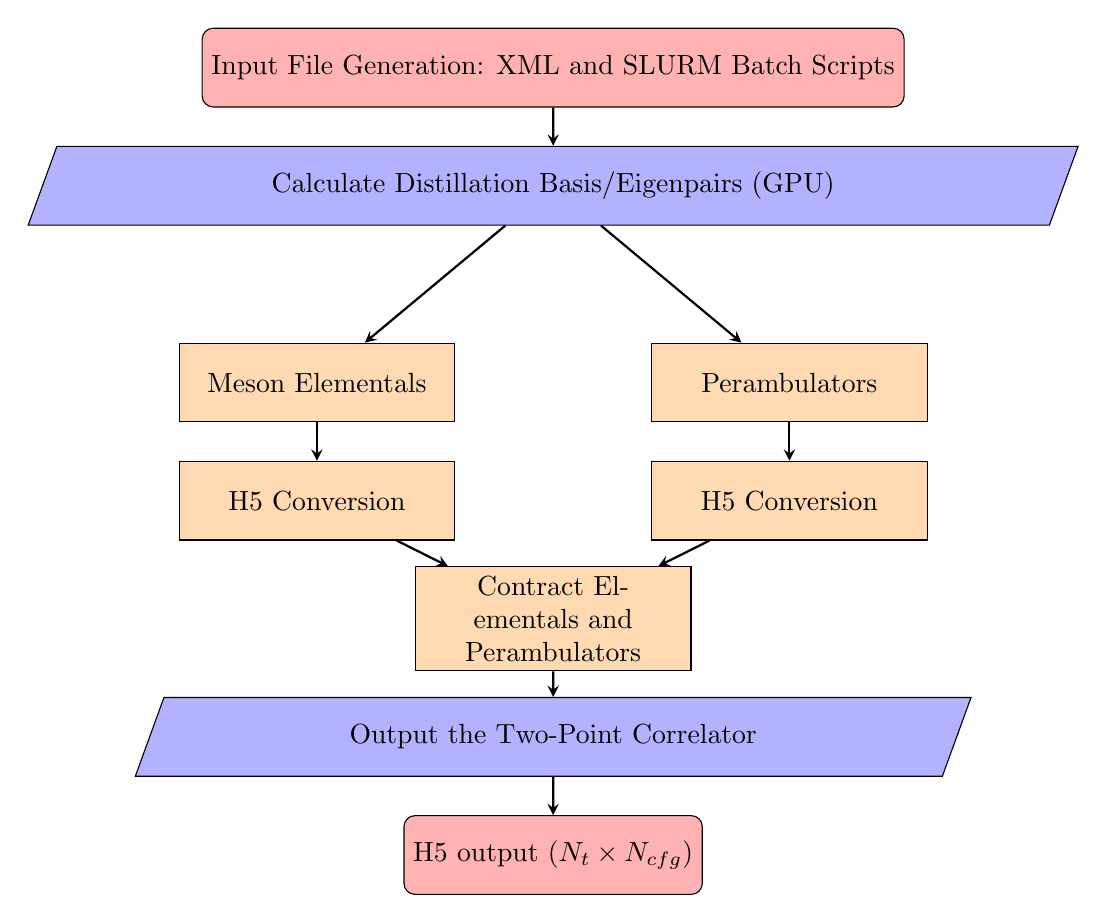
\begin{tikzpicture}[node distance=1.5cm and 3cm] % Adjusted node distance
            \tikzstyle{startstop} = [rectangle, rounded corners, minimum width=3cm, minimum height=1cm, text centered, draw=black, fill=red!30]
            \tikzstyle{io} = [trapezium, trapezium left angle=70, trapezium right angle=110, minimum width=3cm, minimum height=1cm, text centered, draw=black, fill=blue!30]
            \tikzstyle{process} = [rectangle, minimum width=3.5cm, minimum height=1cm, text centered, text width=3cm, draw=black, fill=orange!30]
            \tikzstyle{arrow} = [thick,->,>=stealth]

            % Nodes
            \node (start) [startstop] {Input File Generation: XML and SLURM Batch Scripts};
            \node (in1) [io, below of=start] {Calculate Distillation Basis/Eigenpairs (GPU)};
            
            % Parallel processes
            \node (pro1) [process, below of= in1, xshift=-3cm, yshift=-1cm] {Meson Elementals};
            \node (pro2) [process, below of= in1, xshift=3cm, yshift=-1cm] {Perambulators};
            
            % H5 Conversion processes
            \node (h5conv1) [process, below of=pro1] {H5 Conversion};
            \node (h5conv2) [process, below of=pro2] {H5 Conversion};
            
            % Contracting
            \node (contract) [process, below of=h5conv1, xshift=3cm] {Contract Elementals and Perambulators};
            
            % Output
            \node (out1) [io, below of=contract] {Output the Two-Point Correlator};
            \node (stop) [startstop, below of=out1] {H5 output ($N_t \times N_{cfg}$)};

            % Arrows
            \draw [arrow] (start) -- (in1);
            \draw [arrow] (in1) -- (pro1);
            \draw [arrow] (in1) -- (pro2);
            \draw [arrow] (pro1) -- (h5conv1);
            \draw [arrow] (pro2) -- (h5conv2);
            \draw [arrow] (h5conv1) -- (contract);
            \draw [arrow] (h5conv2) -- (contract);
            \draw [arrow] (contract) -- (out1);
            \draw [arrow] (out1) -- (stop);
        \end{tikzpicture}
      }
    \end{center}
    \caption{Flowchart of the computational workflow for computing lattice objects with distillation.}
    \label{fig:alg_flow}
\end{figure}
\section{Algebraic Multigrid Methods in LQCD}

\subsection{Eigenpairs/Distillation Basis Calculation}
This is the first step in the calculation which is input data for the generation of elementals and perambulators. We use the \verb|Primme| eigensolver to obtain the eigenpairs(eigenvalues,eigenvectors) of the Hermitian Wilson-Dirac operator\cite{PRIMME}\cite{Frommer:2020ovr}. 

The Dirac equation 
\begin{align}
  \mathcal{D}\psi + m \cdot \psi = \eta
\end{align}


\subsection{Elementals Calculation}

\subsection{Perambulators Calculation}

\section{Cost and Storage of Distillation}
% \cite{romero_efficient_2020}.
      \vspace{1em}
       
       % The product of        %  \texttt{max_tslices_in_contraction} \texttt{max_moms_in_contraction} and \texttt{max_vecs} controls how much memory is used for contractions. Their tuning is more critical when using GPUs. The optimal value is usually the largest values of the parameters that the CPU or device can handle.
        % \begin{table}
         \begin{minipage}{16cm}
        \hspace*{2em}\begin{tabular}{ccc}
        Computation    & Operations cost & Memory footprint \\ \hline
        Distillation basis\footnote{Generate colorvector matrix elements}& $N^3Tn^3D$         & $N^3nT$      \\
        Meson elementals\footnote{Contract two matrices $\to$ tensor} & $N^3Tn^3$      & $N^3n + n^3$  \\
        Perambulators\footnote{Projection of the inverse Dirac operator $\to$ square matrices} & $N^3Tn$   & $N^3Tn$            \\
        Contractions\footnote{Contract together matrix elements and perambulators}   & $n^4T$    & $n^{3}T$   
        \end{tabular}
        \end{minipage}
        once a suitable set of perambulators compute, \textbf{reuse} to correlate a collection of interpolators
        
In order to perform spectroscopy calculations for a given ensemble, there exists a sequential dependency chain:
\begin{itemize}
     \setlength\itemsep{1em}
        \item[\checkmark] \textbf{Ensemble generation:} $N_f = 2+1$ quark flavors, a tree level Symanzik improved gluon action and 6-stout dynamical smeared Wilson fermions
        \item[\checkmark] \textbf{HPC Tasks:} Generation of distillation basis, perambulators, meson elementals using \texttt{Chroma} with \texttt{superbblas} support on the Jureca cluster at JSC
        \item Construct \textbf{Di-meson distilled operators} using Hadspec method of subduction coefficents and helicity operators
        \item[\checkmark] Perform \textbf{contractions} of multi-hadron operators $\to$ 2pt correlators
        \item Construct correlation function coming from the \textbf{GEVP} in the right irreducible representation
        \item \textbf{Compute spectrum} and energy shifts w.r.t to the $DD^*$ threshold for a heavy quark mass close to the charm quark mass.
        \item \textbf{L\"uscher analysis} to obtain finite volume energies from Scattering amplitudes
        \item \textbf{Search for Poles} AKA when an attractive potential is not deep enough to hold a bound state
    \end{itemize}

  \section{Contractions}
  We must ``tie" together the perambulators and elementals with some Dirac gamma structure, where we isolate the channel of interest ($J^{PC}$ continuum quantum numbers) with the lattice group representation. For a single meson correlator, \\ 

  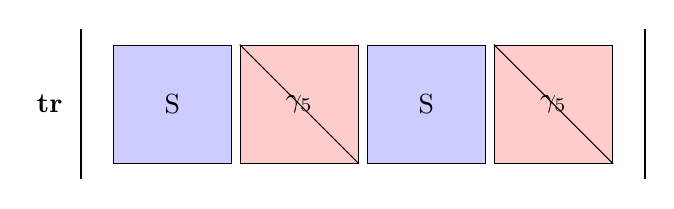
\begin{tikzpicture}[node distance=0.1cm]  % Minimal space between nodes
    \node (box1) [draw, fill=blue!20, minimum width=1.5cm, minimum height=1.5cm] {S};
    \node (box2) [draw, fill=red!20, minimum width=1.5cm, minimum height=1.5cm, right=of box1] {$\gamma_5$};
    \node (box3) [draw, fill=blue!20, minimum width=1.5cm, minimum height=1.5cm, right=of box2] {S};
    \node (box4) [draw, fill=red!20, minimum width=1.5cm, minimum height=1.5cm, right=of box3] {$\gamma_5$};
    
    % Draw diagonal slash through box 2
    \draw (box2.north west) -- (box2.south east);
    
    % Draw diagonal slash through box 4
    \draw (box4.north west) -- (box4.south east);
    
    % Draw the "tr" label
    \node at ($(box1.west) + (-0.8,0)$) {\textbf{tr}};
    
    % Draw large brackets around the first and last boxes
    \draw[thick] 
        ($(box1.north west) + (-0.4, 0.2)$) -- ($(box1.south west) + (-0.4, -0.2)$); % left bracket
    \draw[thick] 
        ($(box4.north east) + (0.4, 0.2)$) -- ($(box4.south east) + (0.4, -0.2)$);  % right bracket
  \end{tikzpicture}
  \\ 

\begin{tikzpicture}[node distance=0.08cm]
  
  % Part 2: Sequence of shapes (rectangles and squares), colored and skinnier
  \node (vrect1) [draw, fill=green!20, minimum width=0.3cm, minimum height=2cm, below=1.5cm of box1, anchor=west] {$V$};
  \node (hrect1) [draw, fill=green!20, minimum width=2cm, minimum height=0.5cm, right=of vrect1] {$V^\dagger$};
  \node (square1) [draw, fill=blue!20, minimum width=1.5cm, minimum height=1.5cm, right=of hrect1] {S};
  
  \node (vrect2) [draw, fill=green!20, minimum width=0.3cm, minimum height=2cm, right=of square1] {$V$};
  \node (hrect2) [draw, fill=green!20, minimum width=2cm, minimum height=0.5cm, right=of vrect2] {$V^\dagger$};
  \node (square2) [draw, fill=red!20, minimum width=1.5cm, minimum height=1.5cm, right=of hrect2] {$\gamma_5$};
  
  \node (vrect3) [draw, fill=green!20, minimum width=0.3cm, minimum height=2cm, right=of square2] {$V$};
  \node (hrect3) [draw, fill=green!20, minimum width=2cm, minimum height=0.5cm, right=of vrect3] {$V^\dagger$};
  \node (square3) [draw, fill=blue!20, minimum width=1.5cm, minimum height=1.5cm, right=of hrect3] {S};

  \node (vrect4) [draw, fill=green!20, minimum width=0.3cm, minimum height=2cm, right=of square3] {$V$};
  \node (hrect4) [draw, fill=green!20, minimum width=2cm, minimum height=0.5cm, right=of vrect4] {$V^\dagger$};
  \node (square4) [draw, fill=red!20, minimum width=1.5cm, minimum height=1.5cm, right=of hrect4] {$\gamma_5$};
  % Draw diagonal slash through box 2
  \draw (square2.north west) -- (square2.south east);
    
  % Draw diagonal slash through box 4
  \draw (square4.north west) -- (square4.south east);

  % Draw large brackets around the first and last boxes
  % Draw the "tr" label
  \node at ($(vrect1.west) + (-0.8,0)$) {$\rightarrow$\textbf{tr}};
  \draw[thick] 
  ($(vrect1.north west) + (-0.4, 0.2)$) -- ($(vrect1.south west) + (-0.4, -0.2)$); % left bracket
  \draw[thick] 
  ($(square4.north east) + (0.2, 0.4)$) -- ($(square4.south east) + (0.2, -0.4)$);  % right bracket
  
\end{tikzpicture}
\\
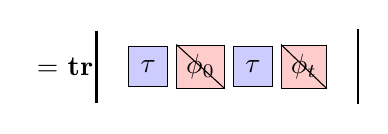
\begin{tikzpicture}[node distance=0.1cm]  % Minimal space between nodes

  \node (box1) [draw, fill=blue!20, minimum width=0.5cm, minimum height=0.5cm] {$\tau$};
  \node (box2) [draw, fill=red!20, minimum width=0.5cm, minimum height=0.5cm, right=of box1] {$\phi_0$};
  \node (box3) [draw, fill=blue!20, minimum width=0.5cm, minimum height=0.5cm, right=of box2] {$\tau$};
  \node (box4) [draw, fill=red!20, minimum width=0.5cm, minimum height=0.5cm, right=of box3] {$\phi_t$};
  
  \draw (box2.north west) -- (box2.south east);
  
  \draw (box4.north west) -- (box4.south east);
  
  \node at ($(box1.west) + (-0.8,0)$) {= \textbf{tr}};
  
  \draw[thick] 
      ($(box1.north west) + (-0.4, 0.2)$) -- ($(box1.south west) + (-0.4, -0.2)$); % left bracket
  \draw[thick] 
      ($(box4.north east) + (0.4, 0.2)$) -- ($(box4.south east) + (0.4, -0.2)$);  % right bracket
\end{tikzpicture}
\\
\noindent
\textbf{tr} 
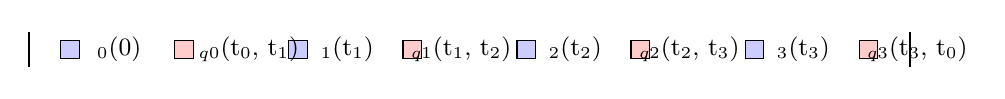
\begin{tikzpicture}[baseline={(current bounding box.center)}, node distance=1.2cm] % Minimal space between nodes

  % Define smaller boxes without internal labels
  \node (box0) [draw, fill=blue!20, minimum width=0.2cm, minimum height=0.2cm] {};
  \node (box_q0) [draw, fill=red!20, minimum width=0.2cm, minimum height=0.2cm, right=of box0] {};
  \node (box1) [draw, fill=blue!20, minimum width=0.2cm, minimum height=0.2cm, right=of box_q0] {};
  \node (box_q1) [draw, fill=red!20, minimum width=0.2cm, minimum height=0.2cm, right=of box1] {};
  \node (box2) [draw, fill=blue!20, minimum width=0.2cm, minimum height=0.2cm, right=of box_q1] {};
  \node (box_q2) [draw, fill=red!20, minimum width=0.2cm, minimum height=0.2cm, right=of box2] {};
  \node (box3) [draw, fill=blue!20, minimum width=0.2cm, minimum height=0.2cm, right=of box_q2] {};
  \node (box_q3) [draw, fill=red!20, minimum width=0.2cm, minimum height=0.2cm, right=of box3] {};
  
  % Attach the subscript and time labels to the right of the boxes
  \node at ($(box0.east) + (0.5, 0)$) {\small $_0(0)$};
  \node at ($(box_q0.east) + (0.7, 0)$) {\small $_{q0}$(t$_0$, t$_1$)};
  \node at ($(box1.east) + (0.5, 0)$) {\small $_1$(t$_1$)};
  \node at ($(box_q1.east) + (0.5, 0)$) {\small $_{q1}$(t$_1$, t$_2$)};
  \node at ($(box2.east) + (0.5, 0)$) {\small $_2$(t$_2$)};
  \node at ($(box_q2.east) + (0.5, 0)$) {\small $_{q2}$(t$_2$, t$_3$)};
  \node at ($(box3.east) + (0.5, 0)$) {\small $_3$(t$_3$)};
  \node at ($(box_q3.east) + (0.5, 0)$) {\small $_{q3}$(t$_3$, t$_0$)};
  
  % Draw large brackets around the first and last boxes
  \draw[thick] 
      ($(box0.north west) + (-0.4, 0.1)$) -- ($(box0.south west) + (-0.4, -0.1)$); % left bracket
  \draw[thick] 
      ($(box_q3.north east) + (0.4, 0.1)$) -- ($(box_q3.south east) + (0.4, -0.1)$);  % right bracket

\end{tikzpicture}
where are $4N_v \times 4N_v$ matrices. A contraction must be carrried out for every gauge configuration (we use 200 in this study); On each configuration, every timeslice and time source is accessed ($N_t = 96$,  $#t_{src} = 24)$ 





\section{Ensemble Details}
We generated ensembles with $N_f = 2+1$ quark flavors, with 6-stout dynamical smeared Wilson fermions and a tree-level Symanzik improved gluon action. Having several $a$ and $m_{\pi}$ at our disposal permit a systematic study of $m_{\pi}$ dependence. Since the doubly charmed tetraquark of interest is close to $D^0D^0\pi^+$ threshold, it is sensitive to $m_{ud}$, thus, it is advantageous to have many ensembles. 
We are using the action and parameters already employed and tuned for Ref. \cite{Durr:2008zz}. 

\begin{tabular}{ccccccc}
\multirow{5}{*}{\substack{$\beta = 3.30$\\ \quad$a = 0.125[fm]$ }} & & $m_{ud}$ & $m_{s}$ & $L^3 \times T$ & $m_\pi$ [MeV] & $N_{conf}$\\
\cmidrule{3-5} \cmidrule{6-7}
& & $-0.1309$ & $-0.057$ & $48^3\times64$ & $135$ & * \\
& & $-0.1291$ & $-0.057$ & $32^3\times64$ & $200$ & * \\
& & $-0.1265$ & $-0.057$ & $24^3\times64$ & $280$ & 1000 \\
& & $-0.1233$ & $-0.057$ & $24^3\times64$ & $330$ & 1000 \\
& & $-0.1200$ & $-0.057$ & $16^3\times64$ & $400$ & 1000 \\
\midrule
\multirow{5}{*}{\substack{$\beta = 3.57$\\ \quad {$a = 0.085[fm]$} }} && $m_{ud}$ & $m_{s}$ & $L^3 \times T$ & $m_\pi$ [MeV] & $N_{conf}$\\
\cmidrule{3-5} \cmidrule{6-7}
& & $-0.0498$ & $-0.007$ & $64^3\times96$ & $135$ & * \\
& & $-0.0483$ & $-0.007$ & $48^3\times64$ & $200$ & 400 \\
& & $-0.0440$ & $-0.007$ & $32^3\times64$ & $300$ & 400 \\
& & $-0.0380$ & $-0.007$ & $24^3\times64$ & $420$ & 400 \\
\midrule
\multirow{5}{*}{\substack{$\beta = 3.70$ \\ \quad $a = 0.065[fm]$}} && $m_{ud}$ & $m_{s}$ & $L^3 \times T$ & $m_\pi$ [MeV] & $N_{conf}$\\
\cmidrule{3-5} \cmidrule{6-7}
& & $-0.02981$ & $-0.0$ & $64^3\times96$ & $135$ & * \\
& & $-0.02855$ & $-0.0$ & $64^3\times96$ & $200$ & * \\
& & $-0.0250$ & $-0.0$ & $40^3\times96$ & $300$ & 400 \\
& & $-0.0220$ & $-0.0$ & $32^3\times96$ & $380$ & 400 \\
& & $-0.0200$ & $-0.0$ & $32^3\times96$ & $420$ & 400 \\
\end{tabular}



% !TEX root = mythesis.tex

%==============================================================================
\chapter{Interpolating Operators}
\label{sec:ops}
%==============================================================================

The overarching aim of hadron spectroscopy on the lattice is to simulate hadrons that we observe in collider experiments. It is advantageous in lattice QCD studies to generate a large basis of interpolating operators to achieve maximal overlap with energy levels of interest. Distillation allows us to restrict this basis to maximize computational efficiency in both the generation of the fundamental objects (perambulators, elementals) and contractions. We first focus on the zero momentum case then extend this framework to non-zero momentum, eg. mesons in flight. We need to construct operators with the flavor basis $\bar c\bar s ud$, $c\bar s u\bar d$, $cc\bar u\bar d$ and $c\bar c u\bar d$, which create and destory a mesonic state, at some fixed time in Euclidean time. The destruction of the state is executed via a contraction of the creation operator with its adjoint at some later time $t$.  The information we can glean from this is the correlation of operators separated by some time $t$, whereby the transfer matrix eigenstates can be obtained. Moreover, the key difference between lattice and continuum eigenstates is the notion of spin, thus we must work in the circular basis of cartesian-vector-like derivative operators and gamma matrices \cite{Morningstar:2013bda}. Using the preceeding section on correlator function construction from contractions, here we will form local and non-local distilled bilinear operators in different irreps of $O_h$, which will comprise a $N \times N$ matrix of two-point correlation functions for each irrep, the GEVP. The dimension of this matrix is, not surprisingly, the number of operators constructed in the particular irrep, as we cannot mix operators with different continuum quantum numbers. Our test case will be $J^{PC} =0^{-+}$, e.g. a pseudoscalar such as the pion. We will walk through lattice operator construction to create a diqaurk $[\bar{q}q]$ of any spin ($J \in \mathbb{Z}$) and parity $P$ with two quark fields and an insertion of the covariant derivative $\nabla$ with gamma strucutre $\Gamma$, the product of which determines the spin $J$.  
  

\section{Spin on a cubic lattice}
Angular momentum ceases to be a good quantum number on the lattice. Thus, in order to forge a link between conntinuum spin and spin on the lattice, we must transform lattice operators according to irreps of the cubic group $O_h$. This optimizes the signal to noise ratio. Only then can we extract eigenstates of the hamiltonian. The lattice irreps, representing symmetries of the cube, are
\begin{align}
    \Lambda = {A_1,T_1,T_2,E,A_2}
\end{align}
\begin{table}
    \begin{tabular}{ccc}
    $\Lambda$ & $d_{\Lambda}$ & $J$\\ \hline
    $A_1$ & 1 & $0,4,6,\dots$\\
    $A_2$ & 1 & $3,6,7,\dots$\\
    $E$ & 2 & $2,4,5,\dots$\\
    $T_1$ & 3 & $1,3,4,\dots$\\
    $T_2$ & 3 & $2,3,4,\dots$\\ \hline
    \end{tabular}
    \caption{The table shows the single-valued irreducible representations
      $\Lambda$ of the cubic group $O$, together with their dimensions
      $d_\Lambda$ and continuum spin content $J$\protect.\label{tab:irrep}}
    \end{table}

\section{Operators on the lattice}
A hadronic operator is a functional of the lattice fields with supplied quantum numbers. These are the gauge-invariant color singlet objects. The lattice regulator ``breaks'' the $SO(3)$ subgroup to a discrete subgroup. $O,\bar{O}$ mapped into the appropiate Hilbert Space such that the corresponding operators $\hat{O} ,\hat{O^\dagger}$  annihilate and create the particle states of interest. We can identify physically allowed states via the spectral decomposition of propagators of interpolating operators: 
\begin{equation}
\braket{O(n_t)\bar{O(0)}} = \sum_{n}\braket{0|\hat{O}|k} \braket{k|\hat{O^{\dagger}}|0} e^{-n_taE_k}
\end{equation}

It is important to note that different spin and parity correspond to different gamma matrices in the fermionic bilinears. Armed with the continuum version of operators, which are classified via charge conjugation and Lorentz transformations, we can cosntruct our lattice operators. The first step is to perform a Wick rotation so that our operators now reside in euclidean spacetime, then substitute the covariant derivatives with the lattice covariant derivative \cite{G_ckeler_1996}, 
\begin{align}
    \overrightarrow{D_\mu}\psi(x) = \frac{1}{2a}(U_{x,\mu}\psi(x + \hat{\mu}) - U_{x-\hat{\mu},\mu}^\dagger\psi(x - \hat{\mu}))
\end{align}

\section{Meson operators at zero total momentum}
We detail the operator construction for zero total momentum, continuum spin $J^P$ and spin component $m$. In general, a local meson interpolator has the form $O_M(n) = \bar{\psi}^{f_1}(n)\Gamma\psi^{f_2}(n)$ where $\Gamma$ is a monomial of gamma matrices and $f$ are of the exposed flavor indices. In our calculations, the fermions fields $\bar{\psi},\psi$ are smeared with the distillation operator. The ingredients are gauge-covariant derivatives(for local operators this is just $\mathbb{I}$), Dirac matrix $\Gamma$, and the distilled meson elementals and perambulators. We obtain the lattice interpolator from the general(continuum) operator by subducing into irreps of the octahedral group $O_h$. 

% In table 1 of \cite{Cheung_2017}, we have the following for the 0 total momentum states: 
% \begin{table}
%     \begin{tabular}{ccc}
%     $LG$ & $\Lambda^p$ & $J^p$ \\
%     \hline
%     $O_h$ & $T_1^+$ & $1^+$ \\
%     $O_h$ & $A_1^-$ & $0^-$ \\
% \end{tabular}
% \end{table}
Fermion-bilinear operators with continuum spin $J$ and momentum $\vec{p}$ are written like so \cite{Cheung_2017}
    \begin{equation}
    \mathcal{O}^{J,m}(\vec{p},t) = \sum_{\vec{x}} e^{i\vec{p}\vec{x}} \bar{q}(\vec{x},t) [\Gamma \overleftrightarrow{D}\dots \overleftrightarrow{D}]^{J,m}q(\vec{x},t)
\end{equation}
In the most general form,

\begin{equation}
    \mathcal{O}_{\Lambda,\mu}^P(\vec{p}=\vec{0},t) = \sum_{\mu_1,\mu_2,\hat{q}} \mathbb{C}(\vec{p} = \vec{0},\Lambda^P,\mu;\vec{q},\Lambda_1,\mu_1;-\vec{q},\Lambda_2,\mu_2) \Omega^{M_1}_{\Lambda_1,\mu_1}(\vec{q},t) \Omega^{M_2}_{\Lambda_2,\mu_2}(-\vec{q},t)
\end{equation}

\section{Local meson operators}

The simplest interpolating operators are the local fermion bilinears $\bar{\psi}(x)\Gamma\psi(x)$. These are preferred as their corresponding gamma structure is much simpler to implement in the contractions. Local signifies that the quark fields at the source and sink are not spatially displaced on gauge links. However, the only continuum quantum numbers we can access with local operators are $J^{PC} = 0^{-+},0^{++},1^{++},1^{+-},1^{--}$ \cite{Dudek_2008}.

For the single pion case, the gamma structure to be inserted between the elementals and perambulators at times $t_0,t_f$, forming the fermion bilinear are
\begin{itemize}
    \item $\gamma_4\gamma_5$
    \item $\gamma_5$

\end{itemize}

\section{Nonlocal meson operators}
To study orbitally excited mesons (higher spin states) we need to employ derivative operators which characterize spatial displacement of quarks on the lattice. These ``forward-backward" gauge covariant derivatives allow us to access states with higher angular momentum. On the lattice, these derivatives are finite displacements of quark fields connected by the gauge links. We will include zero, single, and double derivative operators. We must ensure that the operators have definite charge conjugation as well as a projection operator within the corresponding irreps \cite{liao2002excitedcharmoniumspectrumanisotropic}. Our simplest operator, representing a gauge-invariant construction of a quark and antiquark located at different sites on the lattice along some path $P$ is 
\begin{align}
    \tilde{\psi}_(x_2)\Pi_P U \Gamma \psi(x_1)
\end{align}
where $\Gamma$ takes one of the following forms depending on the state of interest. To access the $J^{PC}=0^{-+}$ channel, we have a set of three pseudoscalar operators which we can then solve the GEVP for

\begin{tabular}{ccc}
    op. & name & cont. \\
    \hline
    $\gamma^i \mathbb{B}^i$ & $(\rho \times \mathbb{B})_{A_1}$ & $0^{-+}$ \\
    $\gamma^4 \gamma^i \mathbb{B}^i$ & $(\rho_{(2)} \times \mathbb{B})_{A_1}$ & $0^{-+}$ \\
    $\gamma^4 \gamma^5 \gamma^i \nabla^i$ & $(b_1 \times \nabla)_{A_1}$ & $0^{-+}$ \\
    \end{tabular}

The advantage of employing nonlocal operators is to achieve access to states with nonzero orbital angular momentum. We act on local meson operators with gauge covariant lattice displacements on one (source or sink) or both (source and sink), the smeared quark fields of the discretized theory, to produce nonlocal operators. 

\subsection{Derivative operators}
Parallel transport of a lattice field is performed by applying a displacement operator to a quark field.  Let $q(x)$ be a quark field and $D_j^{(p)}$ ai displacement operator that moves the quark field for p lattice sites to the direction j in a covariant manner. Let $U$ be the gauge-link as defined in the previous section.
\begin{align}
    D_j^{(p)} q(x) = U_j(x) U_j(x+j) U_j(x+2j)...U_j(x+(p-1)j) q(x+pj)
\end{align}
with dictionary $x(0), y(1), z(2)$.

Thus, a quark bilinear in its $O_h$ representation is tied together with the spatial path $(x_1 \to x_2$). Our new operator will thus live in a representation determined by the Clebsch-Gordan decomposition of the product of representations \cite{Basak_2005}. The set of operators must have definite charge conjugation and the correct projection operator such that it resides in the proper irrep of the cubic group as dictated by group theory.  

\subsubsection{Single derivative operators}
The general form for single derivative meson operators, in which operators of definite spin can be constructed using the standard $SO(3)$ Clebsch-Gordan coefficients, e.g. for a vector-like gamma matrix and one covariant derivative, operators of $J=0,1,2$ can be formed \cite{Dudek_2010}
\begin{equation}
 (\Gamma \times D^{[1]}_{J=1} )^{J, M} = \sum_{m_1, m_2}\big\langle 1, m_1 ; 1, m_2 \big| J, M
  \big\rangle\,  \bar{\psi} \Gamma_{m_1}
  \overleftrightarrow{D}_{m_2} \psi. \nonumber
\end{equation}
The choice of $\Gamma$ plays a role in setting the parity and charge-conjugation quantum numbers of the operator, where the typical naming convention is given by the lowest lying meson in that particular channel. As noted in the introduction of this chapter, we must distribute the different $M$ components belonging to a meson of spin $J$ into definite cubic(lattice) irreps via the group theoretical process called subduction. This is carried out by linear combinations of the $M$ components for each $J$\cite{Dudek_2010}:
\begin{eqnarray}
{\cal O}^{[J]}_{\Lambda,\lambda} \equiv (\Gamma \times D^{[n_D]}_{\ldots})^J_{\Lambda, \lambda} =  \nonumber\\
& & \sum_M {\cal
     S}^{J,M}_{\Lambda, \lambda}   \; (\Gamma \times
   D^{[n_D]}_{\ldots})^{J,M} \equiv \sum_M {\cal S}^{J,M}_{\Lambda,\lambda} {\cal O}^{J,M}, \nonumber
\end{eqnarray}
where $\lambda$ is the ``row'' of the irrep ($1\ldots\mathrm{dim}(\Lambda)$). 

% \subsubsection{Example for $J=0$}
% As seen in the appendix, since this spin value only subduces into the $A_1$ irrep, $\cal{S}_{A1,1}^{0,0} = 1$. This coefficient would correspond to \todo{example state and operator}

%-------------------------------------------------------------------------------%

\subsubsection{Two derivative operators}

\begin{tabular}{|c|c|}
    \hline
    Operator & Lattice spatial displacement correspondence\\
    \hline
    $\gamma_5 \mathbb{D}^i$ & $[\gamma_5 * (dydz + dzdy), \gamma_5 * (dzdx + dxdz), \gamma_5 * (dxdy + dydx)]$ \\
    \hline
    $\gamma_4 \gamma_5 \mathbb{D}^i$ & $[\gamma_5\gamma_4 * (dydz + dzdy), \gamma_5\gamma_4 * (dzdx + dxdz), \gamma_5\gamma_4 * (dxdy + dydx)]$ \\
    \hline
    $\gamma_5 \mathbb{B}^i$ & $[\gamma_5 * (dydz + -dzdy), \gamma_5 * (dzdx + -dxdz), \gamma_5 * (dxdy + -dydx)]$ \\
    \hline
    $\gamma_4 \gamma_5 \mathbb{B}^i$ & $[\gamma_5\gamma_4 * (dydz + -dzdy), \gamma_5\gamma_4 * (dzdx + -dxdz), \gamma_5\gamma_4 * (dxdy + -dydx)]$ \\
    \hline
    % $\gamma_5 \mathbb{E}^i$ & Correspondence not specified \\
    % \hline
    % $\gamma_4 \gamma_5 \mathbb{E}^i$ & Correspondence not specified \\
    % \hline
\end{tabular}


\subsubsection{Momentum projection}
Although we have not yet implemented non-zero momentum into our analysis suite, we very briefly describe what it will entail \cite{Ueding_thesis}. For non-local operators used to construct mesons in flight, we must ``momentum project" into states of definite momentum, which will reside in some irreducible representation of the octahedral group. We want mesonic states to possess definite spatial momentum on each time slice. Note that it is only necessary to project one of the two interpolators of a correlation function to definite momentum, typically at the sink.
$\tilde{O}(\textbf{p},n_t) = \frac{1}{\sqrt{\Lambda_3}} \sum_{n\in\Lambda_3} O(\textbf{n},nt)e^{-ia\textbf{np}}$ 
At non-zero momentum, $O_h$ is broken down to the little groups of Dicyclic nature, eg. $DiC_2, DiC_4$. The extra ingredient required, in contrast to the zero momentum operators, are subduction coefficients that define the helicity operators. For these, we use the Wigner D-matrices then subduce into the irreps of the little group corresponding to the little group of the total momentum $\vec{P}$. See \cite{Basak_2005},\cite{morningstar_extended_2013} for further information. The crucial piece is that these interpolators for mesons in flight will be put into the GEVP for every relevant irrep. 

\section{Meson-Meson Interpolators}
The global $SU(3)$ color symmetry requires that the minimal irreducible color singlet systems can only be $q\bar{q}$, $qqq$, $gg$, $q\bar{q}g$ etc., which implies that multi-quark systems can only exist as molecular configurations if there are no other binding mechanisms \cite{Abolnikov:2024key}. Moreover, as a consequence of the $SU(3)^C$ coupling rule, the state $QQ\bar{q}\bar{q}$ has a dimeson configuration as well as a diquark-antidiquark configuration \cite{Brambilla:2019esw}\cite{Padmanath_2022}. Due to the $SU(3)_c$ coupling rule, when treating tetraquarks as a dimeson system, $(q\bar{q})(q\bar{q})$, the two possible combinations of dimeson $SU(3)_c$ representations that produce a total color singlet state are $({1_c \otimes 1_c})_{1_c}$ and $({8_c \otimes 8_c})_{1_c}$\cite{Guo:2017jvc}. When the pseudoscalar $D$ and vector $D^*$ are coupled together, the resulting system is $DD^*$ with total angular momentum and parity $J^P = 1^+$. Moreover, the wave function of the tetraquark state $T_{cc}^+$ includes two color singlet channels:
\begin{align}
    DD^* = \frac{1}{\sqrt{2}}(D^{0*}D^+ - D^+D^*), \\
    D^*D^* = \frac{1}{\sqrt{2}}(D^{*0}D^{*+} - D^{*+}D^{*0})
\end{align} 
Meson-meson operators are constructed out of single-meson elementals. For mesons in flight, we need to access the helicity operators.  

In general, \textbf{meson-meson operators} are constructed by forming a product of two single-meson operators with appropriate flavor symmetry: \cite{Junnarkar_2019}
\begin{align}
\mathcal{M}^1(x) &= M_1(x)M_2^*(x) - M_2(x)M_1^*(x) \\
M_{1,2}(x) &= (l_{1,2})^a_\alpha(x) (\gamma_5)_{\alpha\beta} \bar{Q}^a_\beta(x) \\
M_{1,2}^*(x) &= (l_{1,2})^a_\alpha(x) (\gamma_i)_{\alpha\beta} \bar{Q}^a_\beta(x) 
\end{align}

Fermion-bilinear operators with continuum spin $J$ and momentum $\vec{p}$ are written like so \cite{Cheung_2017}
\begin{equation}
\mathcal{O}^{J,m}(\vec{p},t) = \sum_{\vec{x}} e^{i\vec{p}\vec{x}} \bar{q}(\vec{x},t) [\Gamma \overleftrightarrow{D}\dots \overleftrightarrow{D}]^{J,m}q(\vec{x},t)\
\end{equation}
% In the most general form,

% \begin{equation}
%     \mathcal{O}_{\Lambda,\mu}^P(\vec{p}=\vec{0},t) = \sum_{\mu_1,\mu_2,\hat{q}} \mathbb{C}(\vec{p} = \vec{0},\Lambda^P,\mu;\vec{q},\Lambda_1,\mu_1;-\vec{q},\Lambda_2,\mu_2) \Omega^{M_1}_{\Lambda_1,\mu_1}(\vec{q},t) \Omega^{M_2}_{\Lambda_2,\mu_2}(-\vec{q},t)
% \end{equation}
% \newpage
% The interpolators we will consider follow that of ~\cite{Padmanath_2022} in Table I, 
\begin{figure}
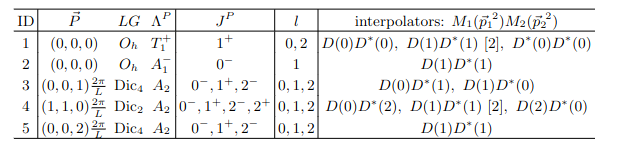
\includegraphics[scale=0.6]{interpolator_table.png}\
\caption{Interpolators along with their total momenta, spatial lattice symmetry group, total spin-parity, and partial wave (of $DD^*$ scattering) that contribute to each irreducible representation}
\end{figure}
\subsection{Distilled Meson-Meson Interpolators}
First, consider the creation and annihilation interpolators for the \(D(0)\) meson with quark content \(c\bar{u}\), \(\bar{c}u\). For smeared quark sources, we can write \cite{peardon_novel_2009} 
\begin{align}
    O(x_0,t_0) &= \Bigg[\sum_{x_1} S_i^{t_0,\alpha_0,a_0}(x_1)^{\alpha_1}_{a_1}\bar{q}^{(f)}(x_1,t)^{\alpha_1}_{a_1}\Bigg] \Gamma^{\alpha_0\beta_0} \Bigg[\sum_{x_2} (S_k^{t_0,\beta_0,a_0}(x_2)^\dagger)^{\alpha_2}_{a_2}\bar{q}^{(f')}(x_2,t)^{\alpha_2}_{a_2}\Bigg] \\
    &= \overline{q_i}(x_0, t)^{\alpha_0}_{a_0} \Gamma^{\alpha_0\beta_0} q_k(x_0,t)^{\beta_0}_{a_0}
\end{align}

Let \(S = \Box\) and Fourier transform into \(p\)-space. 
\[
\overline{\chi}(p, t) = \overline{u}_w(t) \Box_{wx}(t) \cdot e^{-ip\cdot x} \Gamma^A_{xy}(t) \cdot \Box_{yz}(t) c_z(t)
\]

Simplifying the notation (e.g., \(\Gamma^A = e^{-ip\cdot x} \Gamma^A_{xy}(t)\)), we can express the correlation function as 
\begin{align}
C^{2\text{-pt}}(t^\prime, t) &= \braket{\chi(t) \overline{\chi}(t^\prime)} \\
&= \braket{
\overline{c}(t^\prime) \Box(t^\prime) \Gamma^B(t^\prime) \Box(t^\prime) u(t^\prime) \cdot
\overline{u}(t) \Box(t) \Gamma^A(t) \Box(t) c(t)
} \\ 
&= \text{Tr}\left[
    \overline{u}(t^\prime) V(t^\prime) \cdot 
    \underbrace{V^\dagger(t^\prime) \Gamma^B V(t^\prime)}_{\Phi^B(t^\prime)} \cdot 
    V^\dagger(t^\prime) c(t^\prime) \cdot 
    \overline{c}(t) V(t) \cdot 
    \underbrace{V^\dagger(t) \Gamma^A V(t)}_{\Phi^A(t)} \cdot 
    V^\dagger(t) u(t)
\right] \\
&= \text{Tr} \left[\Phi^B(t^\prime) \cdot 
    \underbrace{V^\dagger(t^\prime) c(t^\prime) \overline{c}(t) V(t)}_{\tau_c(t^\prime, t)} \cdot 
    \Phi^A(t) \cdot 
    \underbrace{V^\dagger(t) u(t) \overline{u}(t^\prime) V(t^\prime)}_{\tau_u(t, t^\prime)}
\right] \\
&= \text{Tr}\left[\Phi^A(t) \tau_u(t^\prime, t) \Phi^B(t) \tau_c(t, t^\prime)\right]
\end{align}

Here we have defined the \textbf{perambulator} (including Dirac indices)

\begin{equation}
\tau_q(t^\prime, t)^{\alpha \beta} = V^\dagger(t^\prime) D^{-1}_q(t^\prime, t)^{\alpha \beta} V(t)
\end{equation}

as well as elemental $\Phi$
    
\begin{align}
\Phi^{A, \alpha\beta} 
&= V^\dagger(t) (\Gamma^A)^{\alpha \beta} V(t) \\
&= V^\dagger(t) \mathcal D^A(t)V(t) \mathcal S^{A, \alpha \beta}
\end{align}

where in the second line we have assumed we can decompose \(\Phi\) into terms that act only within coordinate/color space \(\mathcal{D}\) or Dirac spin space \(\mathcal{S}\).

\subsubsection{Distilled Meson-Meson Correlators}
Wick's theorem says that a correlation function is given by the sum of all possible pairs of quark contractions, specifically batched tensor contractions. Given a dimeson operator $[MM']$, we have the following spectral decomposition: 
\begin{align}
    \braket{[MM'](t) [MM']^\dagger(0)} = \sum_{n}^{} |Z_{MM'}^{(n)}|^2 e^{-E_{MM'}^{(n)}t}
\end{align}

As described in the chapter on operator construction, we can form a set of $N$ $MM'$ interpolating operators $$\{[MM']^{(0)},\dots,[MM']^{(N)}\}$$ which have non-trivial overlap with the mesonic state of interest $MM'$. The question is thus, how does one determine the magnitude of the overlaps with the state of interest? Conveniently, the outer product of the set of $N$ interpolating operators acting on itself creates a $N \times N$ matrix of $MM'$ correlators. Not surprisingly, these share the same spectrum. 

In theory, one could fit all $N \times N$ correlators using a simultaneous fit, however, at this point it is standard practice to solve the generalized eigenvalue problem for the set of correlation functions. Solving the following for the eigenvectors $v_n(t,t_0)$ gives us an optimized operator basis
\begin{align}
    C(t)v_n(t,t_0) = \lambda_n(t,t_0)C(t_0)v_n(t,t_0)
\end{align}
Instead of solving the GEVP at the operator level, we deal with the correlation functions directly to yield the optimized correlators 
\begin{align}
    \braket{[MM'](t) [MM']^\dagger(0)} = \sum_{n}^{} |Z_{MM'}^{(n)}|^2 e^{-E_{MM'}^{(n)}t} 
\end{align}


% !TEX root = mythesis.tex

%==============================================================================
\chapter{Mesonic Correlations}
\label{sec:signal}
%==============================================================================
% \newcommand{\todo}[1]{\textbf{\color{red}TODO: #1}}

The meson mass spectrum is extracted via Bayesian analysis of two-point correlation functions. One can systematically improve the agreement with PDG values by using more statistics, employing a collection of ensembles with various quark mass values and lattice spacing. Ultimately, the continuum masses are what we are after. For the study of scattering processes, a Luescher Analysis can be performed in tandem with the spectrum calculations, forging a connection between lattice data and phenomenology. We will briefly walk through the Bayesian fitting approach to extract meson masses, the process by which the ``raw" correlator data is converted into the principal correlator, rotated correlator, or some chosen effective quantity in the optimized basis. 

\section{Basic Correlation Functions}
Given a dimeson operator $[MM']$, we have the following spectral decomposition: 
\begin{align}
    \braket{[MM'](t) [MM']^\dagger(0)} = \sum_{n}^{} |Z_{MM'}^{(n)}|^2 e^{-E_{MM'}^{(n)}t}
\end{align}

As described in \todo{operator section ref }, we can form a set of $N$ $MM'$ interpolating operators(interpolators) $$\{[MM']^{(0)},\dots,[MM']^{(N)}\}$$ which have non-trivial overlap with the mesonic state of interest $MM'$. The question is thus, How does one determine the magnitude of the overlaps with the state of interest? Conveniently, the outer product of the set of $N$ interpolating operators acting on itself creates a $N \times N$ matrix of $MM'$ correlators. Not surpisingly, these share the same spectrum. 

In theory, one could fit all $N \times N$ correlators using a simultaneous fit, however, at this point it is standard practice to solve the generalized eigenvalue problem for the set of correlation functions. Solving the following for the eigenvectors $v_n(t,t_0)$ gives us an optimized operator basis
\begin{align}
    C(t)v_n(t,t_0) = \lambda_n(t,t_0)C(t_0)v_n(t,t_0)
\end{align}
Instead of solving the GEVP at the operator level, we deal with the correlation functions directly to yield the optimized correlators 
\begin{align}
    \braket{[\mathbb{MM'}](t) [MM']^\dagger(0)} = \sum_{n}^{} |Z_{MM'}^{(n)}|^2 e^{-E_{MM'}^{(n)}t} 
\end{align}


$(\bar{\psi}^{f_1}(n)\Gamma\psi^{f_2}(n))^{\dagger} = \pm \bar{\psi}^{f_2} \Gamma \psi^{f_1}$
which can be derived from the fact that the interchange of grassmann variables induces a minus sign and the $\gamma_4$ appears via the relation $\bar{\psi} = \psi^{\dagger}\gamma_4$
TLDR; the conjugate interpolator is obtained by interchanging the $\psi$ and $\bar{\psi}$ and ordering the barred quark fields to the left. 

Now we actually have to evaluate the correlators by employing the property that the fermionic expectation value factorizes with respect to the flavors. We then apply wick's theorem for each of the two flavors, this is **fermion contraction** , by which we obtain the dirac operators. In this case, **only grassmann variables with equal flavor can be contracted with eachother** 

\section{Momentum projection}
For non-local operators used to construct mesons in flight, we must momentum project into states of definite momentum, which will reside in some irreducible representation of the octahedral group. 

We want hadrons tates to be states of definite spatial momentum $\textbf{p}$ 
$\tilde{O}(\textbf{p},n_t) = \frac{1}{\sqrt{\Lambda_3}} \sum_{n\in\Lambda_3} O(\textbf{n},nt)e^{-ia\textbf{np}}$ 

The interpolator is projected to definite spatial momentum and is located on a single time slice $n_t$

Note that it is only necessary to project one of the two interpolators of a correlation function to definite momentum, typically at the sink. 

\section{Signal Saturation with Distillation}

Here we present results for a systematic study of how the signal of the pion two-point correlator with $\vec{p}=(0,0,0)$ is affected by the rank of the distillation basis (number of eigenvectors used) and the number of $t_{src}$ insertions. The sizes of the distillation basis take values in the set $n_{vec}\in {32,64,96,128}$ and the number of $t_{src} \in {1,2,4,8,12,24}$. We perform this study on the ensemble \todo{insert ens info }

The raw correlators after averaging over all $t_{src}$ \todo{insert plot of corrs from corrfit}

The effective masses for each $n_{vec}$: \todo{insert plot}

\subsection{Fits to the $\pi$ correlator}

\subsubsection{$n_{vec}$ dependence}

\todo{insert master pot}
\subsubsection{$t_{src}$ dependence}
\todo{insert master plot}

\subsection{}



% !TEX root = mythesis.tex

%==============================================================================
\chapter{Conclusion}\label{sec:tcc}
% \newcommand{\todo}[1]{\textbf{\color{red}TODO: #1}}

%==============================================================================
\section{Outlook: Towards the Quark Mass Dependence of $T_{cc}(3875)$}
In this section we briefly describe the remaining tasks and the end goals of this project which will comprise a Doctoral thesis. We endeavor to perform a rigorous analysis of the dependence of energy spectra and scattering phase shifts on the degree of distillation smearing. Our testing ground will be the single and double pion system for a collection of covariant derivatives and total momenta. This analysis for hadrons containing charm quarks will then follow suit. In this vein, the remaining tasks are 
\begin{itemize}
    \item computation of meson and doubly charmed spectrum for a range of center-of-mass momenta in various irreps of $O_h$
    \item Finite volume analysis of the discrete spectrum on several volumes and momentum frames
    \item Extract isospin-1 P-wave scattering phase shift 
    \item Determine the systematic uncertainty coming from $m_\pi$ 
    \item $T_{cc}^+$ dependence on $m_\pi$ as the latter approaches the physical point
\end{itemize}
Hadrons containing heavy quarks are prone to discretization errors thus a controlled continuum limit at finite lattice spacing is required!


\subsection{Exotic Hadrons in a (very small) nutshell}
Since the turn of the century, collider experiments have identified resonances that do not fit into the traditional quark model; The two competing hypotheses are that these states are either bound states of di-quarks and anti-di-quarks (tetraquarks) or di-meson states. 
For comprehensive reviews the topic, see \cite{Chen}\cite{Guo:2017jvc} \cite{Brambilla:2019esw}We aim to confirm that the doubly charmed tetraquark state of interest is a member of the class of hadrons shown in g

\begin{figure}[h]
    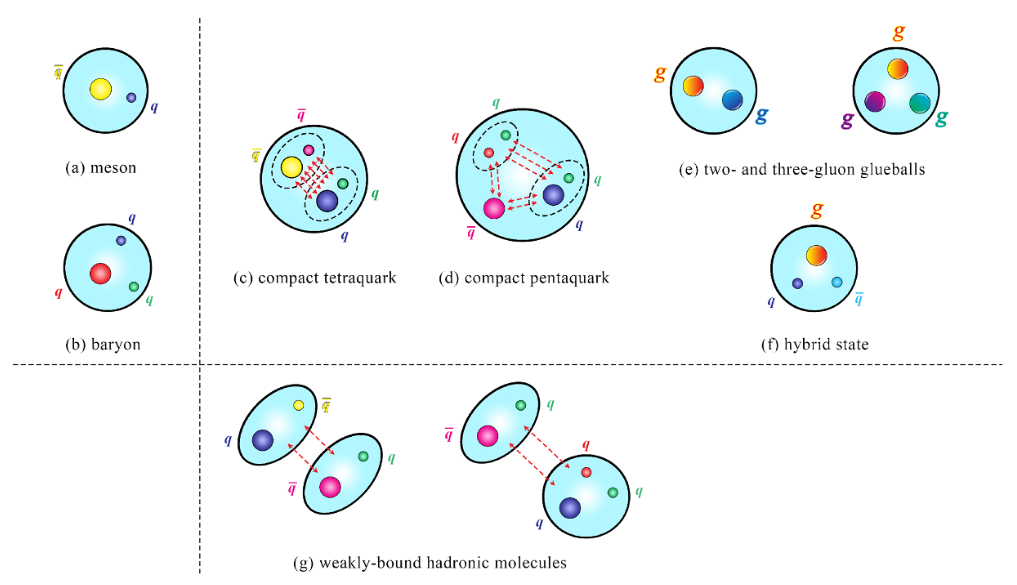
\includegraphics[width=1.0\textwidth]{hadron_states.png}
    \caption{different structures of hadrons with emphasis on the di-meson state in (g) and the tetraquark state in (c)}\label{fig:figure6}
    \end{figure}
The particular color structure of a tetraquark that we will investigate is the hadronic molecule type 
\begin{equation}
    3_q \otimes 3_q \otimes \bar{3}_{\bar{q}} \otimes \bar{3}_{\bar{q}} \rightarrow 1_{[\bar{q}q]_1[\bar{q}q]_1} \rightarrow \delta_{ab} \delta_{cd} \times \bar{q}^aq^b\bar{q}^cq^d 
\end{equation}
Where $a..d = 1..3$ and $n=1...8$ are the color indices. 

The flavor $SU(3)$ representations of the tetraquark states are \cite{sym15071298}
\begin{align}
& 3_q \otimes 3_q \otimes \bar{3}_{\bar{q}} \otimes \bar{3}_{\bar{q}} \nonumber \\
& = (1 \oplus 8)_{[qq]_{\bar{3}}[\bar{q}\bar{q}]_3} \oplus (8 \oplus 10)_{[qq]_6[\bar{q}\bar{q}]_3} \nonumber \\
& \oplus (8 \oplus \bar{10})_{[qq]_{\bar{3}}[\bar{q}\bar{q}]\bar{6}} \oplus (1 \oplus 8 \oplus 27)_{[qq]_6[\bar{q}\bar{q}]_{\bar{6}}}
\end{align} 

\section{Conclusion}
Our goal with this project is to better understand the exotic doubly charmed sector using a data-driven approach with LQCD and distillation in an attempt to dispel disagreement that currently exists in the experimental literature. In Chapter 2 we laid out the formalism for discretizing the continuum theory of QCD and how we transcribe this onto a computer such that we can compute Euclidean correlation functions on all possible gauge field configurations. We motivated our use of distillation smearing with an explanation of traditional quark field smearing methods; This will allow us to efficiently compute the necessary elements for performing hadron spectroscopy calculations, in the form of tensor contractions, while keeping the computational cost low. We laid out the computational considerations of our lattice setup in Chapter 3 and the required software stack to compute eigenpairs, meson elementals, and perambulators using distillation. We highlighted the cost and storage of this method and diagrammatically showed the layout of contracting distilled objects on the lattice to extract physical observables. The construction of a sufficiently large basis of interpolating operators to maximize overlap with energy levels of interest was outlined in Chapter 4. This requires both zero and non-zero values of total momentum and several levels of displacement to access all the spin channels in the continuum. In Chapter 5 we presented our preliminary study on mesonic signal saturation with distillation in order to pin down the optimal parameters to use for the remainder of the ensembles we have at our disposal, namely the rank of the distillation basis and the number of $t_{src}$ insertions. Based on this study, we will generate the rest of our objects using a distillation basis size of 96 and 24 source insertions. Ultimately, this setup will allow us to access the doubly charmed sector and construct di-meson states to extract scattering amplitudes to further probe XYZ states, see the Introduction chapter, with LQCD.  



% \section{Multi-Hadron Interpolating Operators with charm quarks}
% There is a vast amount of literature on computing the Charmonium spectrum with LQCD. See \todo{insert charm cites}

% First, we must calculate the energy levels of the $T_{cc}$, then extract the scattering amplitude and the poles therein. 

% \begin{enumerate}
%     \item compute spectrum for a range of:
%     \subitem center-of-mass momenta 
%     \subitem in various irreducible representations of the relevant symmetry group, which in this case, is the octahedral group $O_h^D$ 
%     \item Perform a finite volume analysis of the discrete spectrum on several mvolumes and momentum frames
%         \subitem \textbf{Note: 
%     \item determine values of the isospin-1 P-wave scattering phase shift 
% \end{enumerate}
    

% Uncomment the following command to get references per chapter.
% Put it inside the file or change \include to \input if you do not want the references
% on a separate page
% \printbibliography[heading=subbibliography]

%------------------------------------------------------------------------------
\appendix
% \part*{Appendix}
% Add your appendices here - don't forget to also add them to \includeonly above
%------------------------------------------------------------------------------
\chapter{Appendix}
\label{sec:app}
%------------------------------------------------------------------------------

\section{Discrete Group Theory}

\section{Conventions}

\subsection{\texttt{Chroma} Euclidean Dirac Matrices}
$\gamma_0 = 
\begin{bmatrix}
    0 & 0 & -1 & 0 \\
    0 & 0 & 0 & -1 \\
    -1 & 0 & 0 & 0 \\
    0 & -1 & 0 & 0 \\
    \end{bmatrix}$
\\
$\gamma_1 = 
\begin{bmatrix}
    0 & 0 & 0 & -i \\
    0 & 0 & -i & 0 \\
    0 & i & 0 & 0 \\
    i & 0 & 0 & 0 \\
    \end{bmatrix}$
\\
$\gamma_2 = 
\begin{bmatrix}
    0 & 0 & 0 & -1 \\
    0 & 0 & 1 & 0 \\
    0 & 1 & 0 & 0 \\
    -1 & 0 & 0 & 0 \\
    \end{bmatrix}$
\\
$\gamma_3 = 
\begin{bmatrix}
    0 & 0 & -i & 0 \\
    0 & 0 & 0 & i \\
    i & 0 & 0 & 0 \\
    0 & -i & 0 & 0 \\
    \end{bmatrix}$
\\
$\gamma_4 = -\gamma_0$ \\
$\gamma_5 = \gamma_0\gamma_1\gamma_2\gamma_3 = 
\begin{bmatrix}
    1 & 0 & 0 & 0 \\
    0 & 1 & 0 & 0 \\
    0 & 0 & -1 & 0 \\
    0 & 0 & 0 & -1 \\
    \end{bmatrix}$
\\
$C = -\gamma_0\gamma_2$

\texttt{Chroma} uses the following conventions \cite{Edwards_2005} For particles of spin-1 can {\em arbitrarily } define a sign convention:
\begin{align}
  \rho(k) &\equiv \bar{\psi} \gamma_k \psi \nonumber \\
  \varrho(k) &\equiv \bar{\psi} \gamma_k \gamma_4 \psi \nonumber\\
  a_1(k) &\equiv \bar{\psi} \gamma_k \gamma_5 \psi \nonumber\\
  b_1(k) &\equiv \bar{\psi}\tfrac{1}{2}  \epsilon_{ijk} \gamma_i \gamma_j \psi \nonumber
\end{align}
With this convention some of the chroma gamma matrices carry a minus sign when creating a state.\\

\vspace{1cm}

\begin{tabular}{c|c|c|c| r| c}
$n_\Gamma(\mathrm{dec})$ & $n_\Gamma(\mathrm{bin})$ & name & $\Gamma$ & state & $\widetilde{n_\Gamma}(\mathrm{dec})$\\
\hline
0 & 0000 & a0 & $1$ & $a_0$ & 15\\
1 & 0001 & rho\_x & $\gamma_1$ & $\rho(x)$ & 14\\
2 & 0010 & rho\_y & $\gamma_2$ & $\rho(y)$ & 13\\
3 & 0011 & b1\_z & $\gamma_1 \gamma_2$ & $b_1(z)$ & 12\\
4 & 0100 & rho\_z & $\gamma_3$ & $\rho(z)$ & 11\\
5 & 0101 & b1\_y & $\gamma_1 \gamma_3$ & $- b_1(y)$ & 10\\
6 & 0110 & b1\_x & $\gamma_2 \gamma_3$ & $b_1(x)$ & 9\\
7 & 0111 & pion\_2 & $\gamma_1 \gamma_2 \gamma_3 = \gamma_5 \gamma_4$ & $\pi$& 8 \\
8 & 1000 & b0 & $\gamma_4$ & $b_0$ & 7 \\
9 & 1001 & rho\_x\_2 & $\gamma_1 \gamma_4$ & $\varrho(x)$ & 6\\
10 & 1010 & rho\_y\_2 & $\gamma_2 \gamma_4$ & $\varrho(y)$ & 5\\
11 & 1011 & a1\_z & $\gamma_1 \gamma_2 \gamma_4 = \gamma_3 \gamma_5$ & $a_1(z)$ & 4\\
12 & 1100 & rho\_z\_2 & $\gamma_3 \gamma_4$ &  $\varrho(z)$ & 3\\
13 & 1101 & a1\_y & $\gamma_1 \gamma_3 \gamma_4 = - \gamma_2 
\gamma_5$ & $- a_1(y)$ & 2\\
14 & 1110 & a1\_x & $\gamma_2 \gamma_3 \gamma_4 = \gamma_1 \gamma_5$ & $a_1(x)$ & 1\\
15 & 1111 & pion & $\gamma_1 \gamma_2 \gamma_3 \gamma_4 = \gamma_5$ &  $\pi$ & 0 \\

\end{tabular}



% \printbibliography[heading=subbibliography]

%------------------------------------------------------------------------------
% Use biblatex for the bibliography
% Add bibliography to Table of Contents
% Comment out this command if your references are printed for each chapter.
\printbibliography[heading=bibintoc]

%------------------------------------------------------------------------------
% Include the following lines and comment out \printbibliography if
% you use BiBTeX for the bibliography.
% If you use biblatex package the files should be specified in the preamble.
% \KOMAoptions{toc=bibliography}
% {\raggedright
%   \bibliographystyle{../refs/atlasBibStyleWithTitle.bst}
%   % \bibliographystyle{unsrt}
%   \bibliography{./thesis_refs,../refs/standard_refs-bibtex}
% }

%------------------------------------------------------------------------------
% Declare lists of figures and tables and acknowledgements as backmatter
% Chapter/section numbers are turned off
\backmatter

\listoffigures
\listoftables

%------------------------------------------------------------------------------
% Print the glossary and list of acronyms
% \printglossaries

%------------------------------------------------------------------------------
% You could instead add your acknowledgements here - don't forget to
% also add them to \includeonly above
% %------------------------------------------------------------------------------
\chapter*{Acknowledgements}
\label{sec:ack}
%------------------------------------------------------------------------------

I would like to thank my advisor Prof.\ Dr.\ Stefan Krieg for giving me the opportunity to pursue my PhD in a beautiful topic and country. He provides endless guidance in both the research vocation and how to navigate the problems that arise when moving to a foreign country. His advice in both realms is always just a door-knock or phone call away and has made my adjustment to Germany, and the frustration-laden process of conducting research, all the more smoother.       

I also wish to thank Dr.\ Giovanni Pederiva for his tireless attention to detail with all things programming, the physics ``big picture'', and advice on how to manage my workflow in an efficient manner. His programming and HPC expertise have been a crucial factor in progressing this project forward. I am indebetted to his patience and suggestions at every step of the way. 

I would be remiss to not acknowledge the fruitful discussions with Dr.\ Evan Berkowitz; His insightful ``mini lectures'' have illuminated countless deep truths in physics and group theory that were previously unbeknownst to me. 


% You should probably use \texttt{\textbackslash chapter*} for
% acknowledgements at the beginning of a thesis and
% \texttt{\textbackslash chapter} for the end.

%%% Local Variables: 
%%% mode: latex
%%% TeX-master: "../mythesis"
%%% End: 


\end{document}
